\chapter{Experiments}
\section{Authentication Scenario:}

In the following Java example the method createDBAccess is used to create a DBAccess object for a database management application.

\begin{lstlisting}
public DBAccess createAccount(String userName, String userType,
 String userPassword) {

		DBAccess access = new DBAccess();
		access.setUserName(userName);
		access.setUserType(userType);
		access.setUserPassword(userPassword);	
				
		return access;
}

\end{lstlisting}

However, there is no authentication mechanism to ensure that the user creating this database user account object has the authority to create new user access. Some authentication mechanisms should be used to verify that the user has the authority to create database access objects.
The following Java code includes a boolean variable and method for authenticating a user. If the user has not been authenticated then the createAccount will not create the database access object.

\begin{lstlisting}

private boolean isUserAuthentic = false;

// authenticate user,
// if user is authenticated then set variable to true
// otherwise set variable to false
public boolean authenticateUser(String username, String password) {
...
}

public DBAccess createAccount(String userName, String userType,
String userPassword) {
			DBAccess access = null;
			
			if (isUserAuthentic) {
			access.setUserName(userName);
			access.setUserType(userType);
			access.setUserPassword(userPassword);
		}
	return access;
}
\end{lstlisting}

Now let's model this kind of scenario in UML statechart considering that for C/C++ application.

\begin{figure}[htbp]
	\centering
	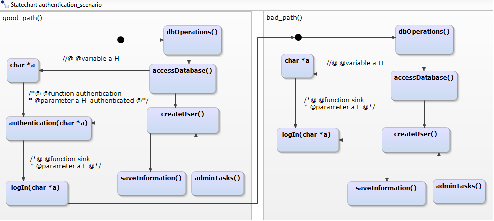
\includegraphics{styles/authentication_scenario.png}
	\caption{Authentication Scenario}
\end{figure}

\section{Declassification Scenario:}
 Noninterference is typically
 too strong a property, most programs use some form of declassification to selectively leak high security information, e.g. when performing a password check or data encryption. Unfortunately, such
 a declassification is often expressed as an operation within a given
 program, rather than as part of a global policy, making reasoning
 about the security implications of a policy more difficult
\begin{figure}[htbp]
	\centering
	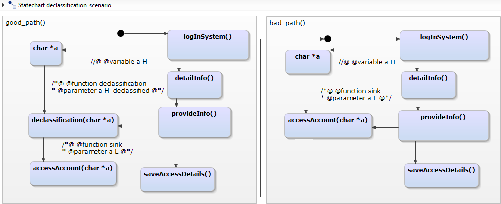
\includegraphics{styles/declassification_scenario.png}
	\caption{Declassification Scenario}
\end{figure}
\section{Sanitization Scenario:}
Web applications are often implemented by developers with limited security skills.As a result, they
contain vulnerabilities. Most of these vulnerabilities stem
from the lack of input validation. That is, web applications
use malicious input as part of a sensitive operation, without having properly checked or sanitized the input values
prior to their use.
In the past research on vulnerability analysis has mostly focused on identifying cases in which a web application directly uses external input in critical operations. However,
little research has been performed to analyze the correctness of the sanitization process. Secured web application helps to prevent the bad guys from gaining unauthorized access to your application/site's data. It helps you keep your data's integrity and ensures availability as needed. Sql injection and XSS attacks are common attacks now-a-days. to prevent this kind of attacks need to use sanitization methods and validate user input properly.\\
This example code intends to take the name of a user and list the contents of that user's home directory. It is subject to the first variant of OS command injection.Example language is in PHP.

\begin{lstlisting}
	$userName = $_POST["user"];
	$command = 'ls -l /home/' . $userName;
	system($command);
\end{lstlisting} 

The userName variable is not checked for malicious input. An attacker could set the userName variable to an arbitrary OS command such as:
\begin{lstlisting}
;rm -rf /
\end{lstlisting}
Then that would prduce a result like this-
\begin{lstlisting}
ls -l /home/;rm -rf /
\end{lstlisting}
Since the semi-colon is a command separator in Unix, the OS would first execute the ls command, then the rm command, deleting the entire file system.

\begin{figure}[htbp]
	\centering
	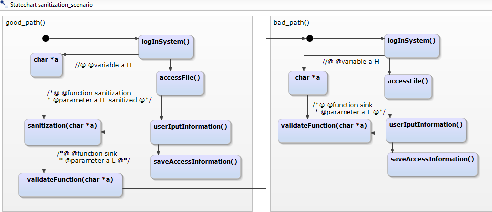
\includegraphics{styles/sanitization_scenario.png}
	\caption{Sanitization Scenario}
\end{figure}